\documentclass{article}
\usepackage[top=2cm,bottom=2cm,left=2cm,right=3.5cm]{geometry}

\usepackage[utf8]{inputenc}
\usepackage{amssymb}
\usepackage{hyperref}
\usepackage{multirow}
\usepackage[most]{tcolorbox}
\tcbuselibrary{skins,breakable}

\newtcolorbox{callout}[2][]{breakable,sharp corners, skin=enhancedmiddle jigsaw,parbox=false,
boxrule=0mm,leftrule=2mm,boxsep=0mm,arc=0mm,outer arc=0mm,attach title to upper,
after title={.\ }, coltitle=purple,colback=purple!10,colframe=purple, title={#2},
fonttitle=\bfseries,#1}

\newtcolorbox{warning}[2][]{breakable,sharp corners, skin=enhancedmiddle jigsaw,parbox=false,
boxrule=0mm,leftrule=2mm,boxsep=0mm,arc=0mm,outer arc=0mm,attach title to upper,
after title={!\ }, coltitle=red,colback=red!10,colframe=red, title={#2},
fonttitle=\bfseries,#1}

\newtcolorbox{esempio}[2][]{breakable,sharp corners, skin=enhancedmiddle jigsaw,parbox=false,
boxrule=0mm,leftrule=2mm,boxsep=0mm,arc=0mm,outer arc=0mm,attach title to upper,
after title={:\ }, coltitle=blue,colback=blue!10,colframe=blue, title={#2},
fonttitle=\bfseries,#1}

\newcommand{\na}[0]{\ensuremath {\overset{N}{\rightarrow}}}
\newcommand{\rl}[3]{\inference{#1}{#2}\text{ #3}}
\newcommand{\bop}[0]{\ensuremath\oplus}
\newcommand{\appl}[2]{\ensuremath(#1)\ #2}
\newcommand{\st}[3][]{\ensuremath{\displaystyle\frac{#3\hfill}{#2\hfill} \text{#1}}}
\newcommand{\N}{\ensuremath \mathbb N}
\newcommand{\I}{\ensuremath \mathbb I}
\newcommand{\lam}[2]{\ensuremath{\lambda#1.#2}}
\newcommand{\inl}[0]{\ensuremath{\ inl\ }}
\newcommand{\inr}[0]{\ensuremath{\ inr\ }}
\newcommand{\case}[3]{\ensuremath{\text{case}#1\ \text{of}\ \left|\begin{aligned}& #2\\ & #3\end{aligned}\right.}}
\newcommand{\Da}[0]{\ensuremath{\Downarrow}}
\newcommand{\while}[2]{\ensuremath{\text{while }#1\text{ do }#2\text{ end}}}
\newcommand{\for}[3]{\ensuremath{\text{for }i=#1\text{ to }#2\text{ do }#3\text{ end}}}
\newcommand{\mE}[0]{\ensuremath{\mathbb{E}}}
\newcommand{\pair}[1]{\ensuremath{\langle#1\rangle}}
\newcommand{\V}{\ensuremath{\mathcal{V}}}
\newcommand{\cE}{\ensuremath{\mathcal{E}}}
\newcommand{\cD}{\ensuremath{\mathcal{D}}}
\newcommand{\cF}{\ensuremath{\mathcal{F}}}
\newcommand{\IF}[0]{\ensuremath {\text{ if }}}
\newcommand{\THEN}[0]{\ensuremath {\text{ then }}}
\newcommand{\ELSE}[0]{\ensuremath {\text{ else }}}
\newcommand{\AND}[0]{\ensuremath {\text{ and }}}
\newcommand{\OR}[0]{\ensuremath {\text{ or }}}
\newcommand{\unpack}[3]{\ensuremath{\text{unpack } #1 \text{ as }\langle #2 \rangle\text{ in }#3}}
\newcommand{\pack}[2]{\ensuremath{\text{pack } \pair{#1} \text{ as } #2 }}
\newcommand{\te}[1]{\text{#1}}
\newcommand{\ls}[0]{\ensuremath{\leadsto^{*}}}
\newcommand{\LET}[0]{\ensuremath{\text{ let }}}
\newcommand{\TIN}[0]{\ensuremath{\text{ in }}}
\newcommand{\NEW}[0]{\ensuremath{\text{ new }}}

\usepackage[parfill]{parskip}

\usepackage{graphicx}
\usepackage{algorithm2e}

\title{Automated Reasoning and Formal Verification}
\author{Diego Oniarti}
\date{Anno 2024-2025}

\begin{document}

\maketitle
\tableofcontents

\section{25-02-2025}
\subsection*{intro}
Slides will be on his \href{https://disi.unitn.it/rseba/DIDATTICA/arfv2025/}{webpage} along with the recordings.

The exam will consist of a script and an oral exam on the topics of the whole course.

\subsection*{boolean/propositional logic}
A propositional \textbf{formula} can be:
\begin{itemize}
    \item $\top$, $\bot$
    \item Propositional \textbf{atoms} $A_1, A_2, \dots, A_n$
    \item A combination of other formulas. If $\varphi_1$ and $\phi_2$ are formulas, so are:
        \begin{itemize}
            \item $\neg \varphi_1$
            \item $\varphi_1\wedge\phi_2$
            \item $\varphi_1\vee\phi_2$
            \item $\varphi_1\to\phi_2$
            \item $\varphi_1\leftarrow\phi_2$
            \item $\varphi_1\leftrightarrow\phi_2$
            \item $\varphi_1\oplus\phi_2$
        \end{itemize}
\end{itemize}

We define a function $Atoms(\varphi)$ representing the set $\{A_1,\dots,A_n\}$ of atoms in $\phi$

A \textbf{clause} is a disjunction of literals $\bigvee_j l_j$ or $(A_1\vee \neg A_2 \vee ...)$

A \textbf{cube} is a conjunction of literals $\bigwedge_j l_j$ or $(A_1\wedge \neg A_2 \wedge ...)$

\subsection*{trees and DAGS}
A tree is a natural representation of an expression, but in the worst cases it can grow exponentially. The same information about the formula can be conveyed by a \textit{Directed Acyclic Graph}, which can grow linearly in size.

\subsection*{Total Truth Assignment}
They can also be abbreviated as \textit{Total Assignment}.\\
A total truth assignment $\mu: Atoms(\varphi)\mapsto\{\top,\bot\}$ represents \textit{one} possible state of the formula.

\subsection*{Partial Truth Assignment}
A partial truth assignment $\mu: \mathcal A \mapsto\{\top,\bot\}, \mathcal A\subset Atoms(\varphi)$ represents $2^k$ total assignments, where $k$ is the number of unassigned literals.

$\mu$ defined for total and partial truth assignments a can be seen as a set of literals (positive and negative ones) or a formula.

\subsection*{Set of models}
$M(\varphi) \triangleq \{\mu | \mu\models\phi\}$ is the set of all models of $\phi$.

\subsection*{Properties}
\begin{itemize}
    \item $\varphi$ is \textit{valid} if every $\mu$ models $\phi$
    \item $\varphi\ \te{valid} \iff \neg\phi\te{ unsatisfiable}$
    \item $\alpha\models\beta \iff \alpha\to\beta\te{ valid}$\marginnote{Deduction theorem}
    \item $\alpha\models\beta \iff \alpha\wedge\neg\beta\ \te{not satisfiable}$\reversemarginpar\marginnote{corollary}
\end{itemize}

\subsection*{Equivalence and Equi-satisfiability}
$\alpha$ and $\beta$ are \textit{equivalent} if $\forall \mu.\mu\models\alpha\iff\mu\models\beta$.\\
In other terms, $M(\alpha)=M(\beta)$.

\textbf{Equi-satisfiability} $M(\alpha)\neq\emptyset \iff M(\beta)\neq\emptyset$. This property is mostly used when applying transformations to formulas $\beta\triangleq T(\alpha)$.

Transformations can be \textit{validity preserving} if they preserve the validity of the formula they're being applied to, or \textit{satisfiability preserving} if they preserve its satisfiability.

\subsection*{Shannon's expansion}
$$\exists v.\varphi := \phi|v=\bot \vee \phi|v=\top$$ The existential is a disjunction between two possible formulas. One where $v$ is set to true, and one where it is set to false.
$$\forall v.\varphi := \phi|v=\bot \wedge \phi|v=\top$$ The universal one is similar, with a conjunction between the two.

\subsection*{Polarity of subformulas}
Polarity is a metric defined for each subformula of a formula $\varphi$ that tells us under how many nested negations it occurs. It can either be positive, negative, or both in some cases.\\
The recursive rules to determine the polarity are shown in the image below
\begin{center}
    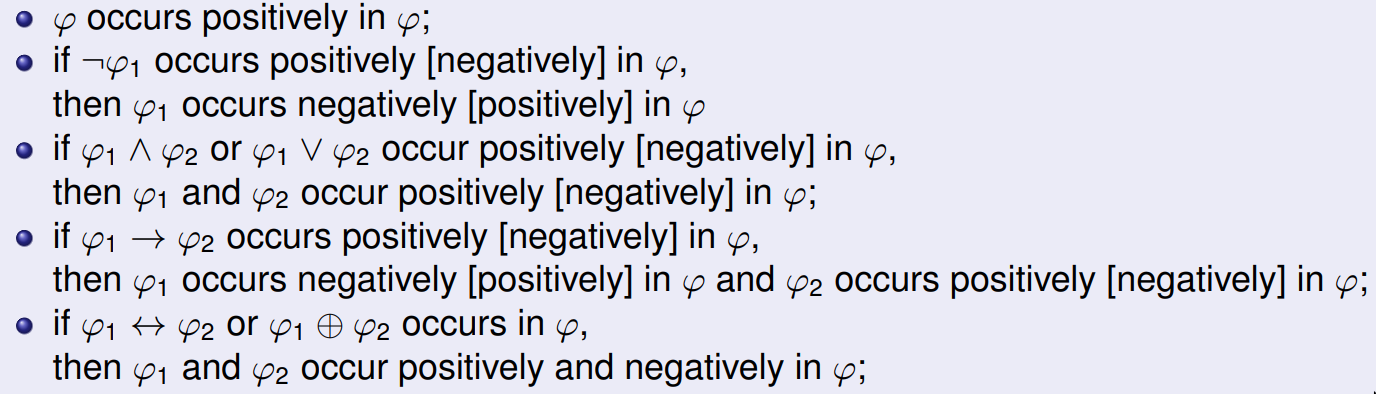
\includegraphics[width=0.8\linewidth]{images/polarity.png}
\end{center}

If we assume $\top=1,\bot=0$ we can also see the polarity of a subformula as "how much it contributes to the overall value of the formula".

\section{Normal forms}
\subsection{Negative Normal Form - NNF}
A negative normal form is a formula in which each negations has been pushed down to the atoms. This implies that every subformula in $NNF(\varphi)$ has positive polarity.

\paragraph{Properties}
\begin{itemize}
    \item Every formula can be made into negative normal form
    \item NNF transformation preserves equivalence
\end{itemize}

\subsection{Conjunctive Normal Form - CNF}
\begin{gather*}
\bigvee_{i=1}^L \bigwedge_{j=1}^{K_i} l_{ij} \\
(l_{11} \wedge l_{12})\vee(l_{21} \wedge l_{22} \wedge l_{23})\vee(...)\vee...
\end{gather*}

Every formula can be converted in \textit{Conjunctive Normal Form}, but there are different ways to do so.

\subsubsection{Naive CNF conversion}
The more intuitive and straightforward method consist of:
\begin{enumerate}
    \item Expanding implications and equivalences
    \item Pushing down negations like in NNF
    \item Recursively applying DeMorgan's rule to get the CNF shape
\end{enumerate}

This method produces a CNF that is \underline{equivalent} to the original formula and \underline{has the same atoms}. It is however rarely used in practical applications because it can be up to \uwave{exponentially} larger than the original formula.

\subsubsection{Labeling CNF conversion}
This is a more efficient \textit{bottom-up} approach, which can be executed while parsing the expression.\\
The main idea is that of introducing new variables that serve as "\textit{labels}" for each subformula. The smaller formulas can be converted to CNF with the naive approach, and then assembled through the labels.

This method introduces new atoms, but $\exists(B_1,\dots,B_k).CNF_l(\varphi)\ \te{equiv}\ \phi$ where $B_1,\dots,B_k$ are the newly introduced variables. This means that $\phi$ and $CNF_l(\phi)$ are equisatisfiable.

The representation obtained from the $CNF_l$ can be reduced  further in size by using polarization to change some implications around.

\section{Basic SAT-solving techniques}
\begin{esempio}{Example}
    A classic problem is that of checking a query under a (usually much larger) knowledge base. This problem can be reduced to SAT. $KB\models\alpha$ or $M(KB)\subseteq M(\alpha)$
    \begin{align*}
        KB\models \alpha \iff SAT(KB \vee \neg \alpha) = false
    \end{align*}
\end{esempio}

\subsection{Intro - Unit propagation}
\paragraph{Resolution rule} Deduction of a new clause from a pair of clauses with \textit{exactly} one incompatible variable (which is called the "\textit{resolvent}").
\begin{align*}
    (\underbrace{a}_\te{common}\vee \underbrace{b}_\te{left}\vee c) \wedge (\underbrace{a}_\te{common}\vee \underbrace{d}_\te{right}\vee \neg c) = (a\vee b\vee d)
\end{align*}
We get $(common \vee left \vee right)$.

\paragraph{Removal of valid clauses}
If a clause is valid (always true) it can be removed from the formula.

\paragraph{Clause subsumption}
If a clause appears on its own and inside another clause, we can remove the second, bigger, clause.
\begin{gather*}
    (\textcolor{purple}{a \vee b}) \wedge (c \vee \textcolor{purple}{a \vee b} \vee d) = (a \vee b)
\end{gather*}

\paragraph{Unit resolution}
Having a clause composed of a single literal forces said literal to be true. This means we can remove all instances of the negated literal.

\paragraph{Unit subsumption}
Like clause subsumption but with a literal instead of a clause.

\paragraph{Unit propagation} Is just the combination of unit resolution and unit subsumption.

These unit propagation rules can happen in a chain. After modifying the formula once we can create new unary clauses for example.

\subsection{Resolution algorithm}
\begin{algorithm}[ht]
    \caption{Resolution algorithm}
    Assume input is in CNF\;
    $\varphi$ is a set of clauses\;
    \CommentSty{//Search for a \textit{refutation} of $\varphi$}\;
    \Repeat{
        a false clause is generated $\vee$ the rule is not applicable
    }{
        apply resolution rule to pairs of clauses\;
    }
\end{algorithm}
This algorithm is correct and complete, but operates in exponential memory and is time inefficient.

\subsection{Tableaux}
Search assignments satisfying $\varphi$ by applying \textit{elimination rules} on its connectors.\\
Try to be clever and put put smaller clauses first in the branching order.\\
The algorithm ends when we reach a leaf (SAT) or we get stuck in every branch (not SAT).\\
A branch is "stuck" when the path to reach it contains both $l$ and $\neg l$.

Tableaux are handy because they only need the elimination rules to be defined and they can be done by hand.
If the formula is in CNF we only really care about the $\vee$ and $\wedge$ elimination rules (respectively $\vee$ branches the formula and $\wedge$ stacks its parts on top of one another).

This is not efficient but it's still better than the resolution-based algorithm. It's also interesting seeing Tableaux as \textit{semantic} resolution methods, since every step keeps memory of the previous ones.

\subsection{DPLL - Davis-Putnam-Longeman-Loveland procedure}
The DPLL procedure tries to build a truth assignment $\mu$ satisfying $\varphi$, and it does this by progressively assigning atoms.
\begin{callout}[blue]{Terminology}
    A literal $l$ is \textit{pure} if it occurs only positively if it occurs only positively
\end{callout}
\begin{wrapfigure}{r}{0.18\textwidth}
    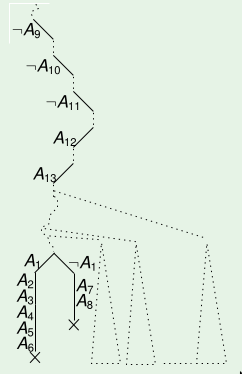
\includegraphics[width=0.18\textwidth]{images/PDLL_waste.png}
    \caption{Example of backtracking wasted search-space}
\end{wrapfigure}
The procedure relies on three rules:
\begin{gather*}
    \begin{array}{lcr}
        \st[Unit]{\varphi [l|\top]}{\varphi \wedge (l)} &
        \st[l pure]{\varphi [l|\top]}{\varphi} &
        \st[split]{\varphi[l|\top]\quad \varphi[l|\bot]}{\varphi}
    \end{array}
\end{gather*}
After setting $l$ to true, for example, remove all clauses containing $l$ and all instances of $\neg l$.

For this technique it is important to find good heuristics when going to choose the next literal.

\subsubsection{Backtracking problem}
The main issue here is the "chronological" backtracking. A DPLL solver stores the assignments of literals on a stack, and once it reaches a dead branch it pops one element from this stack.\\
The issue with this method is that, if the true element to be changed is far into the stack, it will take a long time before reaching it (since it has to explore the whole search space beneath it).

\section{OBDD - Ordered Binary Decision Diagrams}
The OBDD is a canonical representation of boolean formulas. It works as a binary directed acyclic graph, where each node branches setting a variable as $\top$ or $\bot$.\\
The order of the variables is set a priori but it is important since it impacts the size of the OBDD.

\subsection{Generating OBDD - naive}
To generate an OBDD we start from an ordered decision tree (trivial binary tree where each variable is set to both values to explore all configuration).\\
Then we repeatedly apply two reductions:
\begin{itemize}
    \item \textbf{Shared subnodes}: If a subtree occurs twice or more only keep one instance. All the nodes that pointed to the deleted occurrences now point to this one.
        \begin{itemize}
            \item We can use hash consing to identify identical subtrees.
        \end{itemize}
    \item \textbf{Redundancies}: nodes with the same left and right children can be eliminated.
\end{itemize}
Of course this method is extremely expensive, since it has to start from a decision tree.

\subsection{Incremental Building}
\begin{callout}[blue]{if-then-else operator}
    \begin{align*}
        ite(\neg\phi,\varphi^\top,\varphi^\bot) &= ite(\phi,\varphi^\bot,\varphi^\top) \\
        \neg ite\phi,\varphi^\top,\varphi^\bot) &= ite(\phi,\neg\varphi^\top,\neg\varphi^\bot) \\
        ite(\phi,\varphi_1^\top,\varphi_1^\bot) \te{ op } ite(\phi,\varphi_2^\top,\varphi_2^\bot)
                                                &= ite(\phi,\varphi_1^\top\te{ op }\varphi_2^\top,\varphi_1^\bot\te{ op }\varphi_2^\bot) \\
    \end{align*}
    $ite(\phi_1,\varphi_1^\top,\varphi_1^\bot) \te{ op } ite(\phi_2,\varphi_2^\top,\varphi_2^\bot)$ c'è del nesting che non ho voglia di scrivere.
\end{callout}

\begin{align*}
    OBDD(\top,\{A_1,\dots,A_n\}) = 1 & \\
    OBDD(\bot,\{A_1,\dots,A_n\}) = 0 & \\
    OBDD(\varphi,\{A_1,\dots,A_n\}) = ite(& A_1, \\
                                     & OBDD(\varphi[A_1|\top], \{A_2,\dots,A_n\}), \\
                                     & OBDD(\varphi[A_1|\bot],\{A_2,\dots,A_n\}))
\end{align*}

Vedi le slide, le regole sono eterne.

Key points are:
\begin{itemize}
    \item OBDD è canonico. Se due formule sono equivalenti, e usi lo stesso ordinamento di variabili, l'OBDD dell'una e dell'altra sono uguali.
    \item L'ordine delle variabili può fare la differenza tra space complexity lineare e esponenziale.
    \item OBDD è efficiente perché è bottom up.
\end{itemize}

\section{Modern SAT-solving techniques - CDCL}
\textbf{Conflict-Driven Clause-Learning SAT solvers (CDCL)} are non-recursive and avoid the excessive backtracking that slowed PDLL solvers down.\\
The main strengths are:
\begin{itemize}
    \item Conflict-Driven clause learning
    \item random restarts
    \item smart literal selection
    \item smart preprocessing
    \item smart indexing
    \item incremental calls
\end{itemize}

\subsection{Stack representation of truth assignments}
A truth assignment $\mu$ can be represented as a special stack partitioned into \textit{decision levels}.\\
Each decision level contains \textit{one} decision literal and all its \textit{implied literals}.\\
The implied literals keep track of their \textit{antecedent clause}, that is the clause that caused their unit-propagation.

This representation of a truth assignment is equivalent to an \textit{implication graph}.

\subsubsection{Implication graphs}
Implication graphs are Directed Acyclic Graphs where
\begin{itemize}
    \item    each node is a literal, and each edge is labeled with a clause $l_a\overset{c}\mapsto l_b$. 
    \item Decision literals have no incoming edges.
    \item All edges incoming into the same node $l$ must be labeled with the same clause.
    \item $l_1\overset{c}\mapsto l_2 \overset{c}\mapsto \cdots \overset{c}\mapsto l \iff c=(\neg l_1\vee\neg l_2\vee\dots\vee l)$
    \item Conflicts are signaled by the presence of both $l$ and $\neg l$ in the graph.
\end{itemize} 
The intuitive meaning of these rules is that $l_1\overset{c}\mapsto l_2 \overset{c}\mapsto \cdots \overset{c}\mapsto l$ indicates $l$ has been obtained from $l_1,l_2,\dots$ by unit propagation on $c$.
\begin{callout}[purple]{NB}
    The clauses in the chain of implication don't need to be the same.
\end{callout}
\paragraph{UIP - Unique implication point}
An unique implication point is a node $l$ such that \textit{every} path from the last decision to \textit{both} conflict nodes, passes through $l$.\\Trivially the most recent decision node is an UIP.

\subsection{CDCL algorithm}
\begin{algorithm}[ht]
    \caption{CDCL solver}
    status := preprocess($\varphi$,$\mu$)\;
    \While{true}{
        \While{true}{
            status := deduce($\varphi$,$\mu$)\;
            \If{status==SAT}{
                \Return sat\;
            }
            \uIf{status==conflict} {
                \CommentSty{// Backtrack level and conflict set}\;
                $\langle blevel, \eta \rangle$ := analyze\_conflict($\varphi$,$\mu$)\;
                \uIf{blevel==0}{
                    \Return unsat\;
                }\Else{
                    backtrack(blevel,$\varphi$,$\mu$)\;
                }
            }\Else{
                break\;
            }
        }
        decide\_next\_branch($\varphi$,$\mu$)\;
    }
\end{algorithm}
\begin{itemize}
    \item \textbf{preprocess($\varphi$, $\mu$)} simplifies $\varphi$ into an easier equisatisfiable formula, updating $\mu$.
    \item \textbf{decide\_next\_branch($\varphi$, $\mu$)} chooses a new decision literal from $\varphi$ according to some heuristic, and adds it to $\mu$
    \item \textbf{deduce($\varphi$, $\mu$)} performs all deterministic assignments (unit-propagations plus others), and updates $\varphi$, $\mu$ accordingly.
    \item \textbf{analyze\_conflict($\varphi$, $\mu$)} Computes the subset $\eta$ of $\mu$ causing the conflict (conflict set), and returns the “wrong-decision” level suggested by $\eta$ (“0” means that $\eta$ is entirely assigned at level 0, i.e., a conflict exists even without branching)
    \item \textbf{backtrack(blevel,$\varphi$, $\mu$)} undoes the branches up to blevel, and updates $\varphi$, $\mu$ accordingly
\end{itemize}

\subsection{Learning}
We say that the algorithm is "\textit{conflict-driven}" and "\textit{clause-learning}" because whenever a branch fails, we find the conflict set $\eta$ and add $C\overset{def}=\neg\eta$ to the clause set to avoid doing the same mistake again.

We also avoid the PDLL useless backtracking by using $\eta$ to decide the point where to backtrack.

\subsection{Conflict analysis}
\begin{algorithm}[ht]
    \caption{Conflict analysis}
    $C$ := conflicting clause\;
    \Repeat{$C$ meets some criteria}{
        resolve $C$ with the antecedent clause of the last unit-propagated literal $l$ in $C$\;
    }
\end{algorithm}
Some valid criteria are:
\begin{itemize}
    \item \textbf{decision}: $C$ contains only decision literals
    \item \textbf{last UIP}: $C$ contains only one literal assigned at the current decision level and it is the decision literal (the last UIP)
    \item \textbf{first UIP}: $C$ contains only one literal assigned at the current decision level, and it is the first UIP.
\end{itemize}
The first UIP is the better strategy used in modern solvers.

\subsection{Backjumping}
The original strategy for backjumping was to backtrack to the most recent branching point such that the stack did not \textit{fully} contain $\eta$, and then unit propagate the unassigned literal on the conflict clause.

The modern strategy is to backtrack to the highest branching point such that the stack contains \textit{all but one} literals in $\eta$, and then unit propagate the conflict clause like before.

\subsection{Problems with CDCL}
One problem with clause learning is that the solver can generate \textit{a lot} of learned clauses. The solution to this is to remove clauses that are not being used for propagation in a while.\\
A more "lazy" approach is to wait for the clauses to have become too many and to remove the least used ones.

\subsection{Random restarts}
Another technique implemented in CDCL is to randomly restart the search periodically or when some conditions are met. When restarting the learned clauses are kept, and this action can drastically reduce the search space.

\subsection{SAT under assumptions}
We can modify a SAT problem by introducing some assumptions $A\overset{def}=\{l_1,\dots,l_n\}$ and getting $SAT(\varphi,\{l_1,\dots,l_n\})$.

To implement this variant of SAT it is sufficient to put the assumptions as decisions made before decision level 0. This means that whenever the backtrack tries to jump back to one of those, it hits 0 and returns unSAT.

A strong use case for this is to verify the satisfiability of the same formula $\varphi$ repeatedly under different assumptions.

\begin{callout}{property}
    If the \textit{decision} strategy for conflict analysis is used, then $\eta$ is the subset of assumptions causing the inconsistency.
\end{callout}

\subsection{Selection of sub-formulas}
Given a CNF formula $\varphi$ ($\varphi = \bigwedge_{i=1}^n C_i$) and a set of \textit{selectors} $S_1,\dots,S_n$ (fresh boolean atoms), we can use the selectors to "toggle" some clauses so that they may contribute or not to the SAT problem at hand.

The selections are set as \textit{assumptions} and $\varphi$ is modified to make them interact with the rest of the clauses.

\subsection{Incremental SAT solving}
Many modern sat solvers allow to push and pop subformulas onto a base (possibly empty) formula and check the satisfiability at every step.\\
By maintaining the state and the learned clauses from the previous steps we can drastically reduce the search space of each subsequent call.

\section{First-Order Logic}
Giunchiglia
\subsection{Theories} 
In formal logic a \textit{theory} is \textbf{a set of axioms}, where each axiom is a FOL closed formula. This is typical used to give a practical \textit{interpretation} to the symbols in the logic.

Another, more practical definition of a theory is \textbf{a set of models} constraining the interpretation of the logic.

\subsection{Satisfiability Modulo Theories - SMT}
SMT is the problem of deciding if a formula is satisfiable under the constraint of some theory or set of theories.

The theories we're most concerned with are:
\begin{itemize}
    \item Equality and uninterpreted functions
    \item Difference logic
    \item Linear arithmetic over the rationals (LRA)
    \item Linear arithmetic over the integers (LIA)
    \item Arrays
    \item Bit Vectors
    \item Non-linear arithmetic over the reals
\end{itemize}

\subsection{SMT Solvers}
We can solve problems of Satisfiability Modulo Theory by expanding on the CDCL solver we've seen already. The high level workflow is:
\begin{enumerate}
    \item Theory atoms are substituted with fresh boolean variables.
    \item A CDCL solver is used to enumerate truth assignments $\mu_i$ on the modified formula
    \item The set of theory atoms is extracted from the assignment
    \item A \textit{theory specific solver} checks only the satisfiability of the theory atoms
    \item If they're sat, good, otherwise return to 2
\end{enumerate}

For this method a couple important things are
\begin{itemize}
    \item The interleaving between CDCL solver and Theory solver
    \item The Theory solver must offer incremental calling
    \item The $\mathcal T$-solver should provide good conflict sets
    \item Semantically equivalent but syntactically different clauses should be merged into one
    \item Early pruning
\end{itemize}

\subsection*{EUF - Equality and Uninterpreted Functions}
Solvers for EUF are based on merge-sets and E-Graphs.
\begin{callout}{E-Graphs}
    Given the set of terms occurring in the formula represented as nodes in a DAG (or term bank):
    \begin{itemize}
        \item if $(t=s)$ then merge the eq classes of $t$ and $s$
        \item if $\forall i\in 1...k. class(t_i)=class(s_i)$ then merge the eq classes of $f(t_1,...,t_k)$ and $f(s_1,...,s_k)$
        \item if $t\neq s$ and $t$ and $s$ belong to the same class, conflict
    \end{itemize}
\end{callout}

\subsection*{DL - Difference logic}
For difference logic we use a variant of the Bellman-Ford algorithm, where conflicts are revealed by negative cycles.

\subsection*{LRA - Linear Arithmetic over the rationals}
For this a variant of the simplex LP algorithm is used. No idea what that is.

\subsection*{LIA - Linear arithmetic over the integers}
This is an NP-complete problem, and is tackled with a mix of various techniques like simplex, branch\&bound, and cutting planes.

\subsection*{AR - Arrays}
This also is a NP-complete problem.\\
Solvers usually use EUF combined with the array axioms:
\begin{enumerate}
    \item $\forall a.\forall i.\forall e (read(write(a,i,e), i) = e)$ \\
        If I write $e$ to a location and then read that same location, I should get $e$
    \item $\forall a. \forall i. \forall j. \forall e. ((i\neq j) \to read(write(a,i,e),j)=read(a,j))$ \\
        If I write in a location $i$, the values in the rest of the array don't change
    \item $\forall a.\forall b. (\forall i.read(a,i)=read(b,i)) \to (a=b))$ \\
        If all the elements in two arrays are equal, the arrays are equal
\end{enumerate}

\subsection{Combination of theories}
WTF

\section{Kripke Models}
The semantic framework for a variety of logics like Modal Logics, Description Logics, and \textit{Temporal Logics}.

The \textbf{practical role} of a Kripke model is to describe \textit{reactive systems}. This means nonterminating systems with infinite behaviors (like communication protocols and circuits).

\subsection{Formal Definition}
A Kripke model $\langle S, I, R, AP, L\rangle$ consists of:
\begin{itemize}
    \item a finite set of states $S$
    \item a set of initial states $I \subseteq S$
    \item a set of transitions $R\subseteq S\times S$
    \item a set of atomic propositions $AP$
    \item a labeling function $L: S\mapsto 2^{AP}$
\end{itemize}

We assume $R$ to be total, so for every state $s$ there exists at least one state $s'$ such that $s,s'\in R$.\\
Sometimes we use variables with discrete bounded values $v_i\in\{d_1,\dots,d_k\}$

\begin{callout}{Remark}
    Unlike with other types of automata, in Kripke models the values of all variables are always assigned in each state
\end{callout}

\begin{center}
    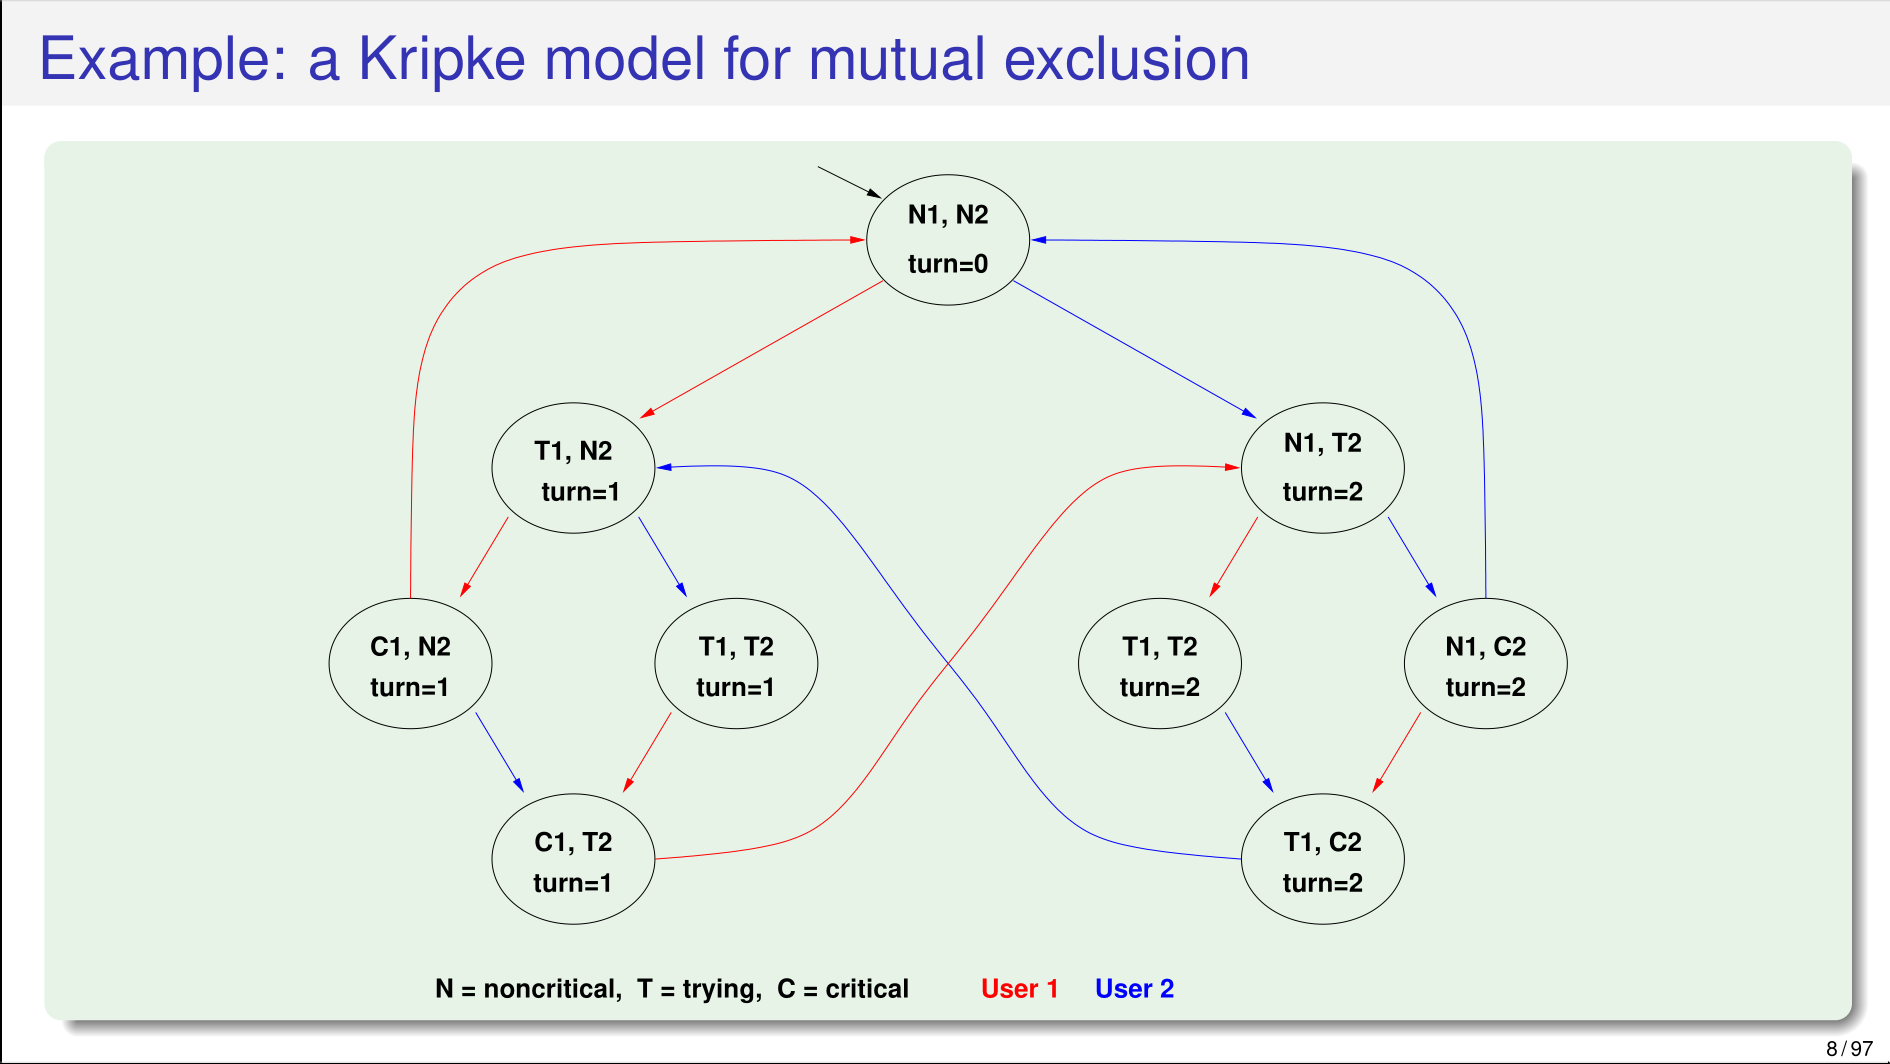
\includegraphics[width=1\linewidth]{images/kripke_example.png}
\end{center}

\paragraph{Path} A path in a Kripke model $M$ is an \textit{infinite} sequence of states $\pi = s_0, s_1, \dots \in S^\omega$

\paragraph{Reachable} A state is reachable if there exists a path that includes it

\paragraph{Asynchronous Composition/Product} At each time instant, one component is selected to perform a transition

It is a typical formalization for protocols since it models agents well.

$M\overset{def}= M_1||M_2\overset{def}= \langle S,I,R,AP,L\rangle$
\begin{itemize}
    \item $S \subseteq s_1\times s_2 \te{ s.t } \forall\langle s_1,s_2\rangle \in S, \forall I \in AP_1\cap AP_2, I\in I_1(s_i) \te{ iff } I \in L_2(s_2)$
    \item $I \subseteq ...$
\end{itemize}
\begin{center}
    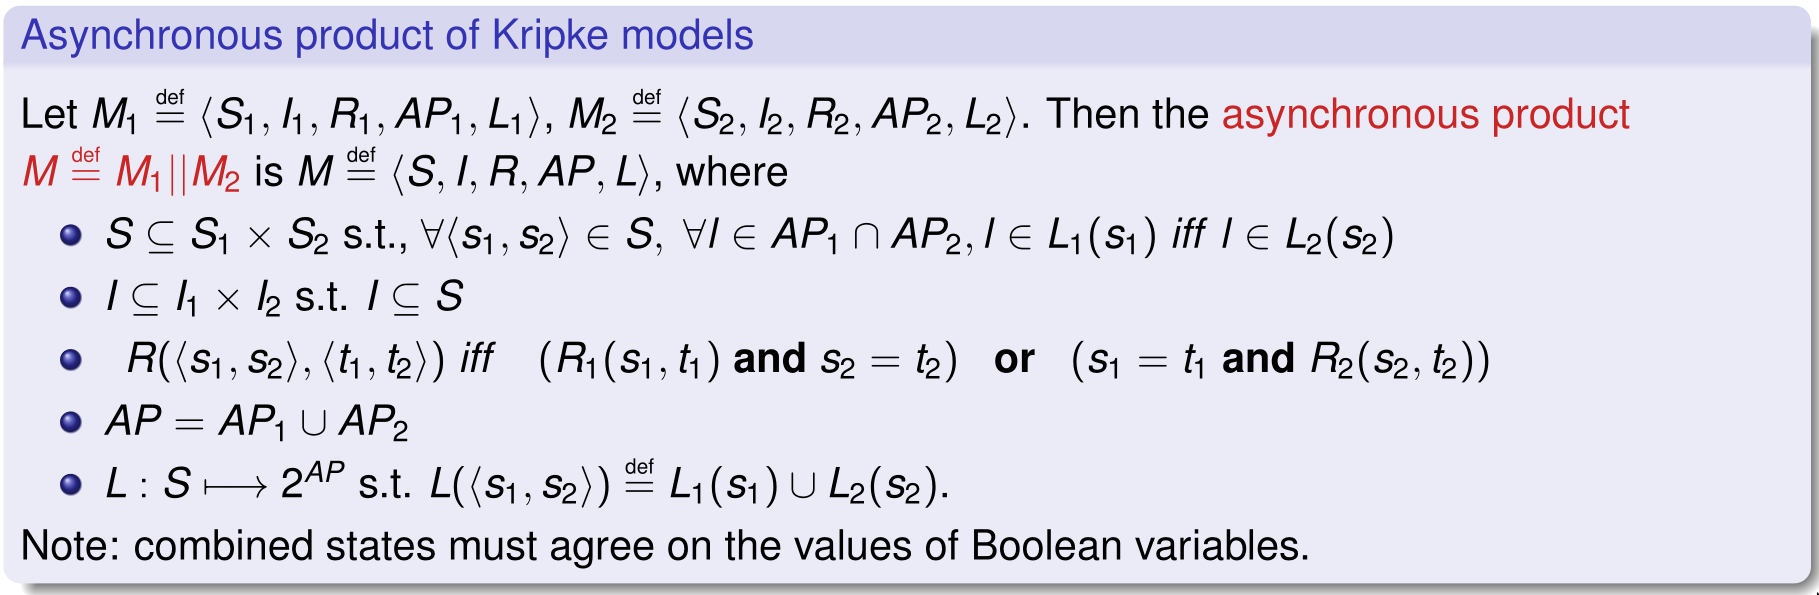
\includegraphics[width=1\linewidth]{images/async_prod.png}
\end{center}

\paragraph{Synchronous Composition/Product} At each time instant, every component performs a transition.

It is a typical formalization for circuits, since it models nicely the behaviour of a clock.
\begin{center}
    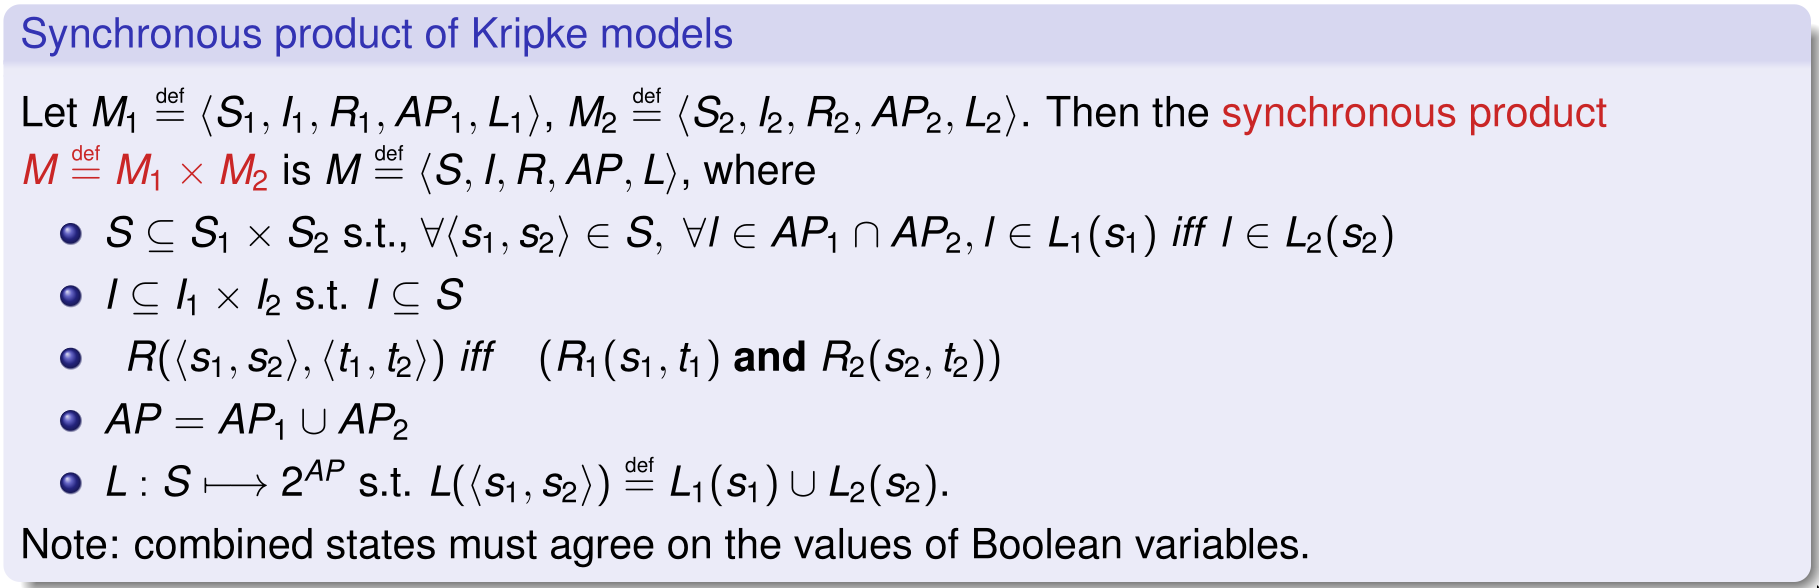
\includegraphics[width=1\linewidth]{images/sync_prod.png}
\end{center}

\subsection{Descriptor languages}
most often a Kripke model is not given explicitly but represented in a structured language (like SMV, VHDL, etc...)

\subsubsection{The SMV Language}
\begin{callout}{riprendere}\end{callout}

\subsection{Standard Programming Languages}
Standard programming languages can be seen as a transition relation in terms also of the program counter.

\subsection{Properties}
\paragraph{Safety Properties}
Bad events never happen (deadlock and other bad conditions). This can be seen as imposing that no reachable state satisfies a "bad" condition (e.g. never two processes in critical section)

This property can be refuted by a finite behaviour (we just need to prove \textit{one} bad execution). This is fairly obvious.

\paragraph{Liveness Properties}
Something desirable will eventually happen. This can be refuted by \textit{infinite} behaviour.\\
Since we're working with finite machines, infinite behaviours are only achieved by loops. Hence they can be detected with (advanced) loop detection.

\paragraph{Fairness Properties}
Something desirable will happen \textit{infinitely often}. This can be seed as a further restriction on the liveness property, since we no longer require that something happens but we require that it also \textit{keeps} happening.

\subsection{Computation trees vs paths}
Given a Kripke structure it's execution can be seen as an infinite set of computation paths or an infinite computations tree
\begin{center}
    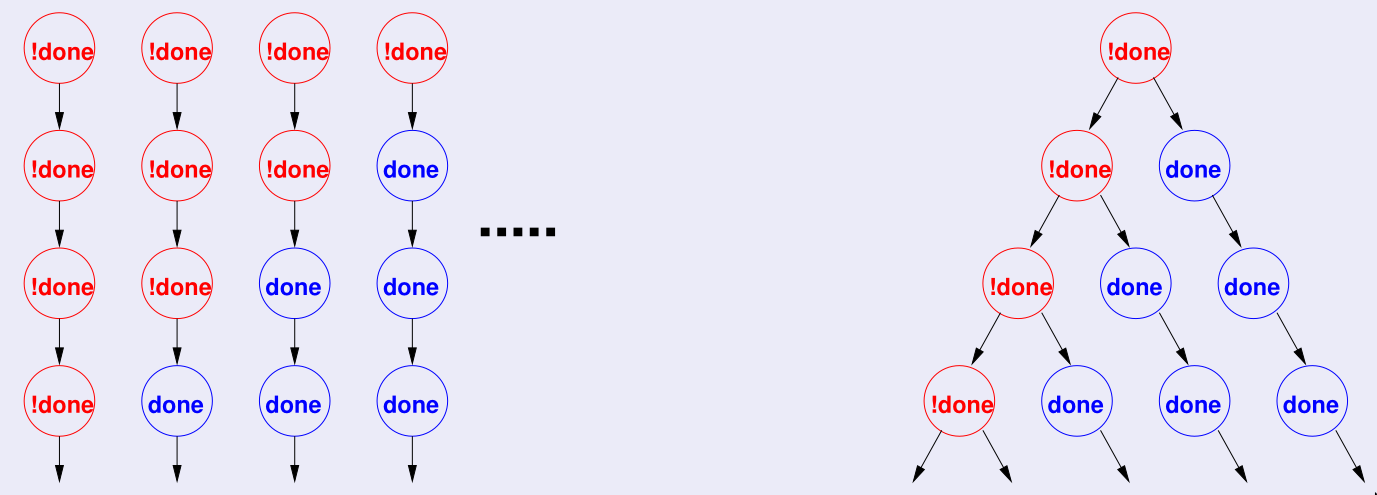
\includegraphics[width=0.8\linewidth]{images/pathVsTree.png}
\end{center}

\section{Temporal Logics}
They are divided in \textit{Linear Temporal Logic (LTL)} and \textit{Computation Tree Logic (CTL)}

\subsection{LTL - Linear Temporal Logic}
An atomic proposition is a LTL formula.\\
Given $\varphi_1, \varphi_2$ LTL, $\neg\varphi_1,\varphi_1\wedge\varphi_2,\dots$ are LTL.\\
$X{\varphi_1}, G{\varphi_1}, F{\varphi_1},\varphi_2 U\varphi_1,\varphi_2 R\varphi_1$ are new operators.
\begin{itemize}
    \item Next \textbf{X}: $X_\varphi$ holds in $s_t$ iff $\varphi$ is true in $s_{t+1}$
    \item Finally (or eventually) \textbf{F}: Is true if $\varphi$ will eventually be true down the path.
\item Globally \textbf{G}: $G\varphi$ is true in $s_t$ iff $\varphi$ is true in all $s_{t'}\geq s_t$
    \item Until $\varphi_1 U \varphi_2$: There is a state in which $\varphi_2$ is true, and up to that state $\varphi_1$ is true
    \item Release $\varphi_1 R \varphi_2$: $\varphi_2$ can become false only if $\varphi_1$ does first
\end{itemize}

\begin{callout}{Fairness}
    \textbf{GF}$\varphi$ is a way to represent fairness, since it indicates that something is gonna happen (F) and that things are always gonna happen (G)
\end{callout}

\paragraph*{Kripke models}
These properties are evaluated over paths (infinite, linear sequences of states) so we can go back to the Kripke model's paths. A model $M$ models $\phi$ if for all paths $\pi$ in $M$, $\pi\models\phi$.

\begin{callout}[red]{NB}
    $M\cancel\models \cancel\implies M\models\neg\phi$
\end{callout}

\subsubsection{Negation Properties}
\begin{wrapfigure}[3]{r}{0.2\textwidth}
    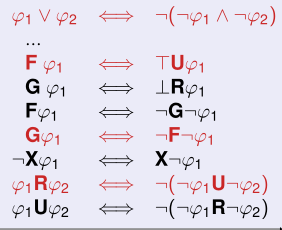
\includegraphics[width=0.2\textwidth]{images/LTLneg.png}
\end{wrapfigure}
From this properties we can see that we only really need $\wedge,\neg,X,U$ to simulate every other connector

\subsubsection{LTL Tableaux rules}
We say that a temporal subformula occurs at top level in $\varphi$ if it occurs in $\varphi$ under the scope of no temporal operator

\begin{callout}[red]{NB}
    $M\models\varphi$ where $\varphi$ does not contain temporal operators, $\varphi$ is only evaluated at the \textbf{initial state}.
\end{callout}

\subsection{CTL - Computation Tree Logic}
As in LTL, we keep the boolean operators and extend them with new ones.
\begin{itemize}
    \item $AX\varphi$
    \item $A(\varphi U \varphi)$
    \item $AG\varphi$
    \item $AF\varphi$
    \item $EX\varphi$
    \item $E(\varphi U \varphi)$
    \item $EG\varphi$
    \item $EF\varphi$
    \item $E(\varphi U \varphi)$
\end{itemize}

The new operators work as "extensions" of the LTL ones:
\begin{itemize}
    \item \textbf{AX}: Necessary next
    \item \textbf{EX}: possible next
    \item \textbf{AF}: necessarily in the future
    \item \textbf{EF}: possible in the future
    \item \textbf{AG}: globally
    \item \textbf{EG}: possible henceforth
    \item \textbf{AU}: necessarily until
    \item \textbf{EU}: possible Until
\end{itemize} 
The \textbf{A} can be seen as "all", so the property holds in all branches.\\
The \textbf{E} can be seen as "exists", so there is at least one branch where the property holds.

\begin{figure}[h]
    \centering
    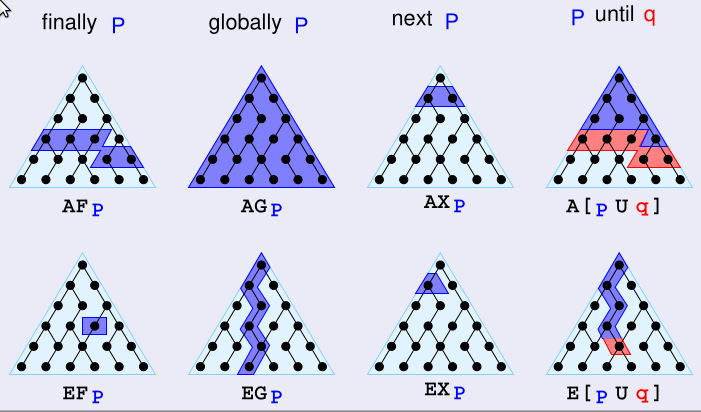
\includegraphics[width=0.5\linewidth]{images/CTLtrees.png}
    \caption{Visual representation of the operators}
\end{figure}

\begin{callout}[red]{Watch out!}
    LTL and CTL are \textbf{NOT} equivalent and none of them is strictly more expressive than the other.\\
    There are LTL formulas that cannot be expressed in CTL and vice versa.
    \begin{center}
        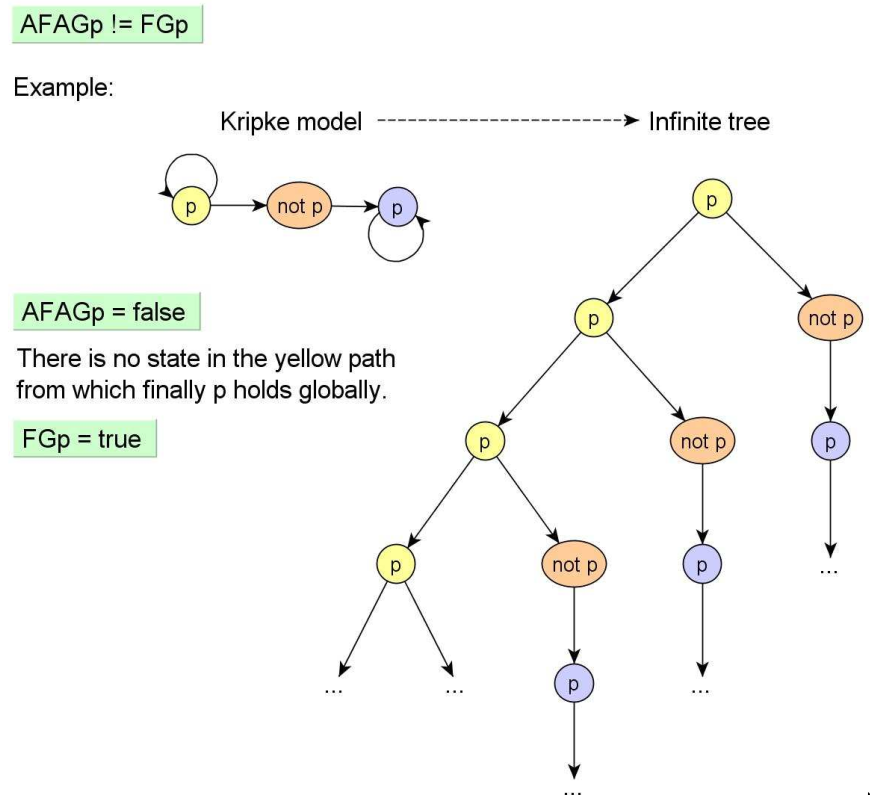
\includegraphics[width=0.5\linewidth]{images/AFAGvsFG.png}
    \end{center}
    There are obviously some formulas that can be expressed in both.
\end{callout}

\subsection{CTL*}
CTL* divides formulas into \textit{state formulae} and \textit{path formulae}.
\paragraph{State formulas} boolean operations and boolean connections of smaller state formulas are state formulas. If $\psi$ is a \textit{path} formula, $A\psi$ and $E\psi$ are state formulas.
\paragraph{Path formulas} State formulas are path formulas. Boolean combinations of path formulas are path formulas. Path/time quantifiers on path formulas are path formulas.

CTL* subsumes both LTL and CTL.
\begin{itemize}
    \item $\varphi$ in CTL $\implies$ $\varphi$ in CTL*
    \item $\varphi$ in LTL $\implies$ A$\varphi$ in CTL*
    \item $LTL \cup CTL \subset CTL*$
\end{itemize}
So CTL* gives us the tools to compare CTL and LTL in one framework.

\section{Automata-Theoretic LTL Reasoning}
\subsection{Infinite word languages}
Given an alphabet $\Sigma$ a $\omega$-word $\alpha$ over $\Sigma$ is an infinite sequence of elements from $\Sigma$.\\
The set of all infinite words is $\Sigma^\omega$\\
A $\Omega$-language $L$ is a collection of $\omega$-words $L\subseteq\Sigma^\omega$.

\subsection{Omega-Automata}
We consider automaton running over infinite words. A word is \textit{accepted} if there is at least one state which is repeated \textit{infinitely} many times.

\subsection{Buchi automata}
A non-deterministic Buchi automaton (NBA) is $(Q,\Sigma,\delta,I,F)$
\begin{itemize}
    \item $Q$ finite set of states
    \item $\Sigma$ finite alphabet
    \item $I\subseteq Q$ set of initial states
    \item $F\subseteq Q$ set of accepting states
    \item $\delta\subset Q\times\Sigma\times Q$ transition relation
\end{itemize}
A deterministic Buchi automaton (DBA) has the same definition except $\delta$ is a function instead of a relation $\delta:Q\times\Sigma\mapsto Q$

\paragraph{Runs and Languages} A run $\rho$ of $A$ on $\omega$-word $\alpha=a_0,a_1,...$ is an infinite sequence $\rho=q_0,q_1,...$ st $q_0\in I$ and $q_i\overset{a_i}\rightarrow q_{i+1}$ for $0\leq i$.

A run $\rho$ is \textit{accepting} if $inf(\rho)\cap F \neq \emptyset$.

The \textit{language} accepted by $A$ is the set of all $\alpha$ accepted by $A$.

\paragraph{DBA vs NBA}
DBAs are strictly \textbf{less} powerful than NBAs.

\subsection{Operations on Buchi Automata}
For the NBAs $A_1, A_2$ we can construct the NBAs for the union of their languages and for their intersection.\\
It is also possible to do complementation but it's hard and out of the scope of this course.

\paragraph{Union}
The size of the union of two automata is $|A| = |A_1| + |A_2|$.\\
To build it we just take the two graphs and consider them together. A graph does not need to be connected, so we can leave them like that.

\paragraph{Intersection}
The size of the intersection of two automata is $|A| \leq |A_1|\cdot|A_2|\cdot 2$.\\
To build the intersection we consider the combination of each state and we add a flag $Q=Q_1\times Q_2 \times \{1,2\}$. The initial states are $I=I_1\times I_2\times \{1\}$ and the final ones are $F=F_1\times F_2\times \{1\}$.

\subsection{LTL and Buchi}
\paragraph{validity and satisfiability}
Let $\psi$ be an LTL formula ($\models \psi$, $\neg\psi$ unsat, $L(A_{\neg\psi})=\emptyset$).\\
$A_{\neg\psi}$ is a Buchi Automatons which represents all and only the paths that satisfy $\neg\psi$ (do not satisfy $\psi$).

\paragraph{Entailment}
Let $\varphi,\psi$ LTL formulas. ($\varphi\models\psi$, $\models\varphi\to\psi$\\
blah blah

\paragraph{LTL model checking}

\subsection{Language emptiness checking}
To check that a language is \textit{not empty} we just need to find and accepting cycle reachable from an initial state. If we find a loop we know we can follow it forever and touch the final state infinite many times.

\subsubsection{Naive Double Nested DFS algorithm}
The easy approach to find such loops is to run two nested DFS over the graph. Whenever the outer DFS finds a final state $f$, the inner one is started. If the inner DFS gets back to $f$, there is a loop.

This method is $O(n^2)$ and is not very good.

\subsubsection{SCC-based algorithm}
We can use the \textit{Strongly Connected Components} of a graph to make the naive implementation run in linear time.

\subsubsection{Smart Double Nested DFS}
The naive method can be improved drastically with two modifications:
\begin{enumerate}
    \item The inner DFS is not started when a final state is encountered, but only when it is popped.
    \item Keep two hash tables and two stacks.
\end{enumerate}

The algorithm is explained better in the slides, the complexity becomes $O(n)$.

\subsection{Kripke Models to Buchi Automata}
We can transform a Kripke model $M=\langle S, S_0, R, L, AP\langle$ into an NBA $A_M=\langle Q,\Sigma,\delta,I,F\rangle$ such that
\begin{itemize}
    \item $Q := S\cup \{init\}$, $init$ being a new initial state
    \item $\Sigma := 2^{AP}$ total truth-assignments as alphabet symbols
    \item $I := \{init\}$
    \item $F:=Q$
    \item $\begin{array}{rl}\delta: & q\xrightarrow{a} q' \iff (q,q')\in R \AND L(q')=a\\
        & init\overset a \rightarrow q \iff q\in S_0 \AND L(q)=a\end{array}$
\end{itemize}

The labels are effectively moved from the nodes to the incoming edges of said nodes.

\subsection{From LTL formulas to Buchi Automata}
\paragraph{LTL Negative Normal Form}
Every LTL formula can be converted into its negative normal form which only uses $\wedge,\vee,X,U,R$ on propositional literals.

\begin{callout}{Reminder}
    A property of NNF is that every non atom in $\varphi$ occurs positively.
\end{callout}

\paragraph{On-the-fly construction of $A_\varphi$}
\begin{enumerate}
    \item Apply the tableau expansion rules to $\varphi$
        \begin{gather*}
            \psi_1 U \psi_2 \implies \psi_2 \vee (\psi_1\wedge X(\psi_1 U \psi_2)) [\AND F\psi\implies\psi \vee XF\psi] \\
            \psi_1 R \psi_2 \implies \psi_2 \wedge (\psi_1\vee X(\psi_1 R \psi_2)) [\AND G\psi\implies\psi \wedge XG\psi] 
        \end{gather*}
    \item Convert all formulas into \textit{disjunctive normal form}\\
        This is the counterpart to the conjunctive normal form, where $\wedge$ and $\vee$ are inverted
    \item huh?
\end{enumerate}

\section{CTL Model Checking}



\end{document}
